\documentclass[]{article}
\usepackage{lmodern}
\usepackage{amssymb,amsmath}
\usepackage{ifxetex,ifluatex}
\usepackage{fixltx2e} % provides \textsubscript
\ifnum 0\ifxetex 1\fi\ifluatex 1\fi=0 % if pdftex
  \usepackage[T1]{fontenc}
  \usepackage[utf8]{inputenc}
\else % if luatex or xelatex
  \ifxetex
    \usepackage{mathspec}
  \else
    \usepackage{fontspec}
  \fi
  \defaultfontfeatures{Ligatures=TeX,Scale=MatchLowercase}
\fi
% use upquote if available, for straight quotes in verbatim environments
\IfFileExists{upquote.sty}{\usepackage{upquote}}{}
% use microtype if available
\IfFileExists{microtype.sty}{%
\usepackage{microtype}
\UseMicrotypeSet[protrusion]{basicmath} % disable protrusion for tt fonts
}{}
\usepackage[margin=1in]{geometry}
\usepackage{hyperref}
\hypersetup{unicode=true,
            pdftitle={How to keep it togetheR},
            pdfauthor={Marc A.T. Teunis, Ph.D. - Hogeschool Utrecht, Lab. Innovative Testing},
            pdfborder={0 0 0},
            breaklinks=true}
\urlstyle{same}  % don't use monospace font for urls
\usepackage{color}
\usepackage{fancyvrb}
\newcommand{\VerbBar}{|}
\newcommand{\VERB}{\Verb[commandchars=\\\{\}]}
\DefineVerbatimEnvironment{Highlighting}{Verbatim}{commandchars=\\\{\}}
% Add ',fontsize=\small' for more characters per line
\usepackage{framed}
\definecolor{shadecolor}{RGB}{248,248,248}
\newenvironment{Shaded}{\begin{snugshade}}{\end{snugshade}}
\newcommand{\KeywordTok}[1]{\textcolor[rgb]{0.13,0.29,0.53}{\textbf{#1}}}
\newcommand{\DataTypeTok}[1]{\textcolor[rgb]{0.13,0.29,0.53}{#1}}
\newcommand{\DecValTok}[1]{\textcolor[rgb]{0.00,0.00,0.81}{#1}}
\newcommand{\BaseNTok}[1]{\textcolor[rgb]{0.00,0.00,0.81}{#1}}
\newcommand{\FloatTok}[1]{\textcolor[rgb]{0.00,0.00,0.81}{#1}}
\newcommand{\ConstantTok}[1]{\textcolor[rgb]{0.00,0.00,0.00}{#1}}
\newcommand{\CharTok}[1]{\textcolor[rgb]{0.31,0.60,0.02}{#1}}
\newcommand{\SpecialCharTok}[1]{\textcolor[rgb]{0.00,0.00,0.00}{#1}}
\newcommand{\StringTok}[1]{\textcolor[rgb]{0.31,0.60,0.02}{#1}}
\newcommand{\VerbatimStringTok}[1]{\textcolor[rgb]{0.31,0.60,0.02}{#1}}
\newcommand{\SpecialStringTok}[1]{\textcolor[rgb]{0.31,0.60,0.02}{#1}}
\newcommand{\ImportTok}[1]{#1}
\newcommand{\CommentTok}[1]{\textcolor[rgb]{0.56,0.35,0.01}{\textit{#1}}}
\newcommand{\DocumentationTok}[1]{\textcolor[rgb]{0.56,0.35,0.01}{\textbf{\textit{#1}}}}
\newcommand{\AnnotationTok}[1]{\textcolor[rgb]{0.56,0.35,0.01}{\textbf{\textit{#1}}}}
\newcommand{\CommentVarTok}[1]{\textcolor[rgb]{0.56,0.35,0.01}{\textbf{\textit{#1}}}}
\newcommand{\OtherTok}[1]{\textcolor[rgb]{0.56,0.35,0.01}{#1}}
\newcommand{\FunctionTok}[1]{\textcolor[rgb]{0.00,0.00,0.00}{#1}}
\newcommand{\VariableTok}[1]{\textcolor[rgb]{0.00,0.00,0.00}{#1}}
\newcommand{\ControlFlowTok}[1]{\textcolor[rgb]{0.13,0.29,0.53}{\textbf{#1}}}
\newcommand{\OperatorTok}[1]{\textcolor[rgb]{0.81,0.36,0.00}{\textbf{#1}}}
\newcommand{\BuiltInTok}[1]{#1}
\newcommand{\ExtensionTok}[1]{#1}
\newcommand{\PreprocessorTok}[1]{\textcolor[rgb]{0.56,0.35,0.01}{\textit{#1}}}
\newcommand{\AttributeTok}[1]{\textcolor[rgb]{0.77,0.63,0.00}{#1}}
\newcommand{\RegionMarkerTok}[1]{#1}
\newcommand{\InformationTok}[1]{\textcolor[rgb]{0.56,0.35,0.01}{\textbf{\textit{#1}}}}
\newcommand{\WarningTok}[1]{\textcolor[rgb]{0.56,0.35,0.01}{\textbf{\textit{#1}}}}
\newcommand{\AlertTok}[1]{\textcolor[rgb]{0.94,0.16,0.16}{#1}}
\newcommand{\ErrorTok}[1]{\textcolor[rgb]{0.64,0.00,0.00}{\textbf{#1}}}
\newcommand{\NormalTok}[1]{#1}
\usepackage{graphicx,grffile}
\makeatletter
\def\maxwidth{\ifdim\Gin@nat@width>\linewidth\linewidth\else\Gin@nat@width\fi}
\def\maxheight{\ifdim\Gin@nat@height>\textheight\textheight\else\Gin@nat@height\fi}
\makeatother
% Scale images if necessary, so that they will not overflow the page
% margins by default, and it is still possible to overwrite the defaults
% using explicit options in \includegraphics[width, height, ...]{}
\setkeys{Gin}{width=\maxwidth,height=\maxheight,keepaspectratio}
\IfFileExists{parskip.sty}{%
\usepackage{parskip}
}{% else
\setlength{\parindent}{0pt}
\setlength{\parskip}{6pt plus 2pt minus 1pt}
}
\setlength{\emergencystretch}{3em}  % prevent overfull lines
\providecommand{\tightlist}{%
  \setlength{\itemsep}{0pt}\setlength{\parskip}{0pt}}
\setcounter{secnumdepth}{0}
% Redefines (sub)paragraphs to behave more like sections
\ifx\paragraph\undefined\else
\let\oldparagraph\paragraph
\renewcommand{\paragraph}[1]{\oldparagraph{#1}\mbox{}}
\fi
\ifx\subparagraph\undefined\else
\let\oldsubparagraph\subparagraph
\renewcommand{\subparagraph}[1]{\oldsubparagraph{#1}\mbox{}}
\fi

%%% Use protect on footnotes to avoid problems with footnotes in titles
\let\rmarkdownfootnote\footnote%
\def\footnote{\protect\rmarkdownfootnote}

%%% Change title format to be more compact
\usepackage{titling}

% Create subtitle command for use in maketitle
\newcommand{\subtitle}[1]{
  \posttitle{
    \begin{center}\large#1\end{center}
    }
}

\setlength{\droptitle}{-2em}

  \title{How to keep it togetheR}
    \pretitle{\vspace{\droptitle}\centering\huge}
  \posttitle{\par}
  \subtitle{\emph{List-columns in a dataframe}}
  \author{Marc A.T. Teunis, Ph.D. - Hogeschool Utrecht, Lab. Innovative Testing}
    \preauthor{\centering\large\emph}
  \postauthor{\par}
      \predate{\centering\large\emph}
  \postdate{\par}
    \date{Last update: 2019-01-28 13:27:13}


\begin{document}
\maketitle

\section{Demo for the Utrecht University R Cafe, 28 January
2019}\label{demo-for-the-utrecht-university-r-cafe-28-january-2019}

\subsection{What is R to me?}\label{what-is-r-to-me}

\begin{itemize}
\tightlist
\item
  Every day go-to for analytics of very different types of data
\item
  Statistical analysis \texttt{\{lme\}}, \texttt{\{lme4\}},
  \texttt{\{nlme\}}
\item
  Genomics \texttt{\{DESeq2\}}, \texttt{\{edgeR\}}, \texttt{\{limma\}},
  \texttt{\{Glimma\}}
\item
  Microbiome analysis \texttt{Bioconductor} \& \texttt{qiime2}
\item
  Interactivity with \texttt{\{Shiny\}} and \texttt{\{flexdashboards\}}
\item
  Reproducibility \texttt{\{rmarkdown\}}, \texttt{\{bookdown\}},
  \texttt{\{blogdown\}}
\item
  Tutorials and teaching \texttt{\{learnr\}}, \texttt{\{reticulate\}} --
  combine Python \& R
\item
  Getting data \texttt{\{plumber\}}, \texttt{\{getGEO\}},
  \texttt{\{rentrez\}}
\item
  Text mining \texttt{\{tidytext\}}, \texttt{\{igraph\}},
  \texttt{\{ggiraph\}}
\item
  Visualizations \texttt{\{ggplot2\}}, \texttt{\{tidygraph\}},
  \texttt{\{gganimate\}}, \texttt{\{tmap\}}
\end{itemize}

\subsection{Content for today}\label{content-for-today}

PART I: Starting with List-columns

\textbf{There is more in this demo than we can cover today}

PART II: MORE LIST-COLUMNS (do-it-yourself)

\subsection{}\label{section}

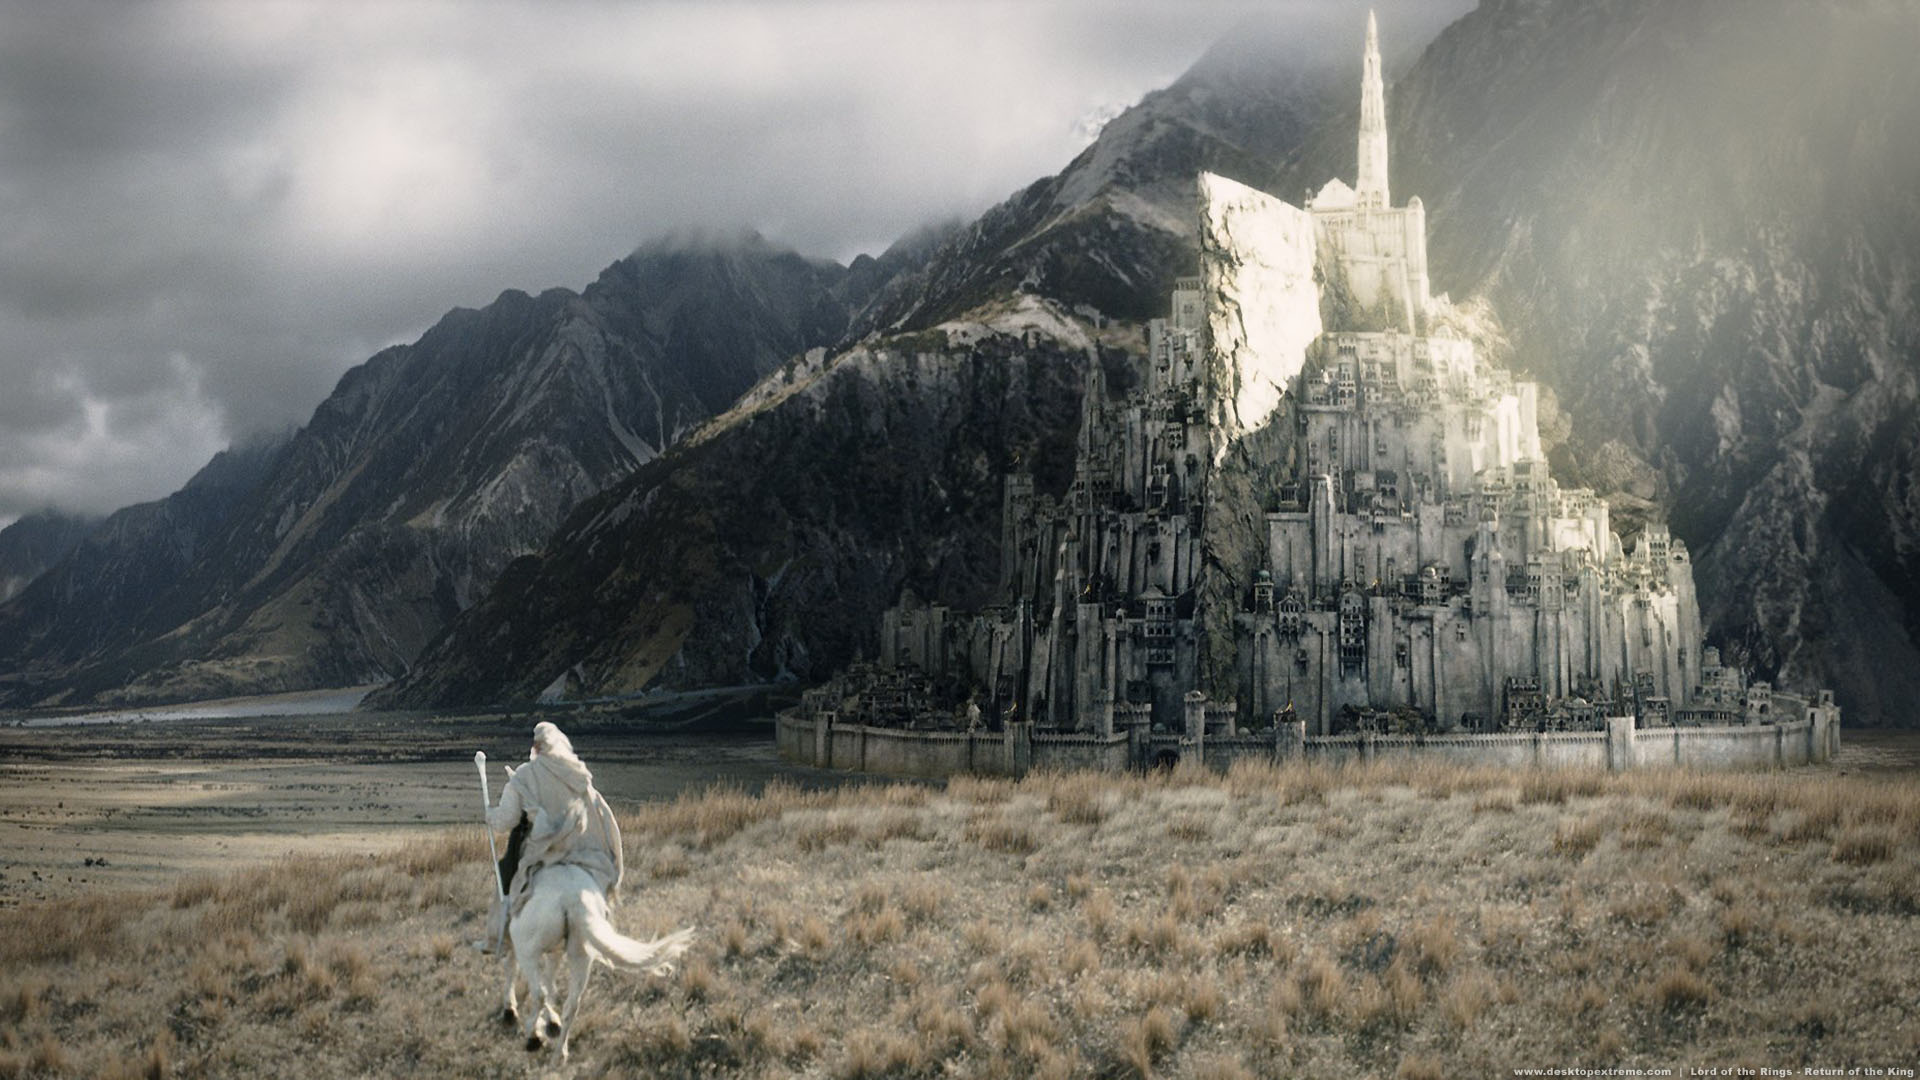
\includegraphics[width=1000px]{/home/marc_teunis/rcafe/images/ground_to_cover}

\subsection{Getting access and
materials}\label{getting-access-and-materials}

Clone the repository to your RStudio Environment from:

\texttt{https://github.com/uashogeschoolutrecht/rcafe} or login

\texttt{http://rserverkcgdl.hudatascience.nl} with

login: \ldots{} passwd: \ldots{}

\subsection{Packages}\label{packages}

The packages used in this tutorial

\begin{Shaded}
\begin{Highlighting}[]
\KeywordTok{library}\NormalTok{(tidyverse)}
\KeywordTok{library}\NormalTok{(modelr)}
\KeywordTok{library}\NormalTok{(lubridate)}
\KeywordTok{library}\NormalTok{(broom)}
\KeywordTok{library}\NormalTok{(purrr)}
\KeywordTok{library}\NormalTok{(repurrrsive)}
\end{Highlighting}
\end{Shaded}

\subsection{Dataframes and lists are recursive
vectors}\label{dataframes-and-lists-are-recursive-vectors}

\begin{Shaded}
\begin{Highlighting}[]
\NormalTok{table1 <-}\StringTok{ }\KeywordTok{tribble}\NormalTok{(}
  \OperatorTok{~}\NormalTok{a,    }\OperatorTok{~}\NormalTok{b,  }\OperatorTok{~}\NormalTok{c,     }\OperatorTok{~}\NormalTok{d, }
  \StringTok{"x"}\NormalTok{,   }\DecValTok{1}\NormalTok{,   }\OtherTok{TRUE}\NormalTok{,   }\FloatTok{1.45}\NormalTok{, }
  \StringTok{"y"}\NormalTok{,   }\DecValTok{2}\NormalTok{,   }\OtherTok{FALSE}\NormalTok{,  }\FloatTok{3.88}\NormalTok{,}
  \StringTok{"z"}\NormalTok{,   }\DecValTok{3}\NormalTok{,   }\OtherTok{TRUE}\NormalTok{,   }\FloatTok{33.5}
\NormalTok{  ) }
\NormalTok{table1}
\end{Highlighting}
\end{Shaded}

\begin{verbatim}
## # A tibble: 3 x 4
##   a         b c         d
##   <chr> <dbl> <lgl> <dbl>
## 1 x         1 TRUE   1.45
## 2 y         2 FALSE  3.88
## 3 z         3 TRUE  33.5
\end{verbatim}

\begin{Shaded}
\begin{Highlighting}[]
\KeywordTok{is.atomic}\NormalTok{(table1}\OperatorTok{$}\NormalTok{a)}
\end{Highlighting}
\end{Shaded}

\begin{verbatim}
## [1] TRUE
\end{verbatim}

\subsection{Column containing a list (in a
dataframe)}\label{column-containing-a-list-in-a-dataframe}

\begin{Shaded}
\begin{Highlighting}[]
\NormalTok{table2 <-}\StringTok{ }\KeywordTok{tribble}\NormalTok{(}
  \OperatorTok{~}\StringTok{ }\NormalTok{a,      }\OperatorTok{~}\NormalTok{b,      }\OperatorTok{~}\NormalTok{c,       }\OperatorTok{~}\NormalTok{d,     }\OperatorTok{~}\NormalTok{e, }
  \StringTok{"x"}\NormalTok{,      }\DecValTok{1}\NormalTok{,       }\OtherTok{TRUE}\NormalTok{,     }\FloatTok{1.45}\NormalTok{,   }\DecValTok{1}\OperatorTok{:}\DecValTok{10}\NormalTok{,}
  \StringTok{"y"}\NormalTok{,      }\DecValTok{2}\NormalTok{,       }\OtherTok{FALSE}\NormalTok{,    }\FloatTok{3.88}\NormalTok{,   }\KeywordTok{c}\NormalTok{(}\OtherTok{TRUE}\NormalTok{, }\OtherTok{FALSE}\NormalTok{),}
  \StringTok{"z"}\NormalTok{,      }\DecValTok{3}\NormalTok{,       }\OtherTok{TRUE}\NormalTok{,     }\FloatTok{33.5}\NormalTok{,   }\StringTok{"Utrecht"}   
\NormalTok{  ) }

\KeywordTok{is.list}\NormalTok{(table2}\OperatorTok{$}\NormalTok{e)}
\end{Highlighting}
\end{Shaded}

\begin{verbatim}
## [1] TRUE
\end{verbatim}

\begin{Shaded}
\begin{Highlighting}[]
\KeywordTok{is.vector}\NormalTok{(table2}\OperatorTok{$}\NormalTok{e)}
\end{Highlighting}
\end{Shaded}

\begin{verbatim}
## [1] TRUE
\end{verbatim}

\subsection{Iterate over a dataframe}\label{iterate-over-a-dataframe}

\begin{Shaded}
\begin{Highlighting}[]
\KeywordTok{map}\NormalTok{(table1, class)}
\end{Highlighting}
\end{Shaded}

\begin{verbatim}
## $a
## [1] "character"
## 
## $b
## [1] "numeric"
## 
## $c
## [1] "logical"
## 
## $d
## [1] "numeric"
\end{verbatim}

\subsection{Iterate over a
list-column}\label{iterate-over-a-list-column}

\begin{Shaded}
\begin{Highlighting}[]
\KeywordTok{map}\NormalTok{(table2}\OperatorTok{$}\NormalTok{e, nchar)}
\end{Highlighting}
\end{Shaded}

\begin{verbatim}
## [[1]]
##  [1] 1 1 1 1 1 1 1 1 1 2
## 
## [[2]]
## [1] 4 5
## 
## [[3]]
## [1] 7
\end{verbatim}

\subsection{Case data}\label{case-data}

Let's switch to RStudio and open the file:

\texttt{demo.Rmd}

\subsection{Data origin}\label{data-origin}

Whooping cough outbreaks from The World Health Organization

\url{http://data.euro.who.int/cisid/?TabID=463987}

See for variable and data collection also:

\url{http://ecdc.europa.eu/sites/portal/files/documents/Pertussis\%20AER.pdf}

for more details see file: ``load\_data.R''

\subsection{Load the tidy version of the
dataset}\label{load-the-tidy-version-of-the-dataset}

The code for cleaning and tidying the data is in the file
``./load\_data.R''

\begin{Shaded}
\begin{Highlighting}[]
\KeywordTok{source}\NormalTok{(}\DataTypeTok{file =} \KeywordTok{file.path}\NormalTok{(root,}
                        \StringTok{"load_data.R"}\NormalTok{))}
  
\KeywordTok{head}\NormalTok{(pertussis_data_tidy, }\DataTypeTok{n =} \DecValTok{2}\NormalTok{)}
\end{Highlighting}
\end{Shaded}

\begin{verbatim}
## # A tibble: 2 x 4
##     key country year       annual_pertussis_cases
##   <dbl> <chr>   <date>                      <int>
## 1     2 Albania 1980-01-01                     NA
## 2     5 Andorra 1980-01-01                     NA
\end{verbatim}

\begin{Shaded}
\begin{Highlighting}[]
\KeywordTok{names}\NormalTok{(pertussis_data_tidy)}
\end{Highlighting}
\end{Shaded}

\begin{verbatim}
## [1] "key"                    "country"               
## [3] "year"                   "annual_pertussis_cases"
\end{verbatim}

\subsection{Overall trend}\label{overall-trend}

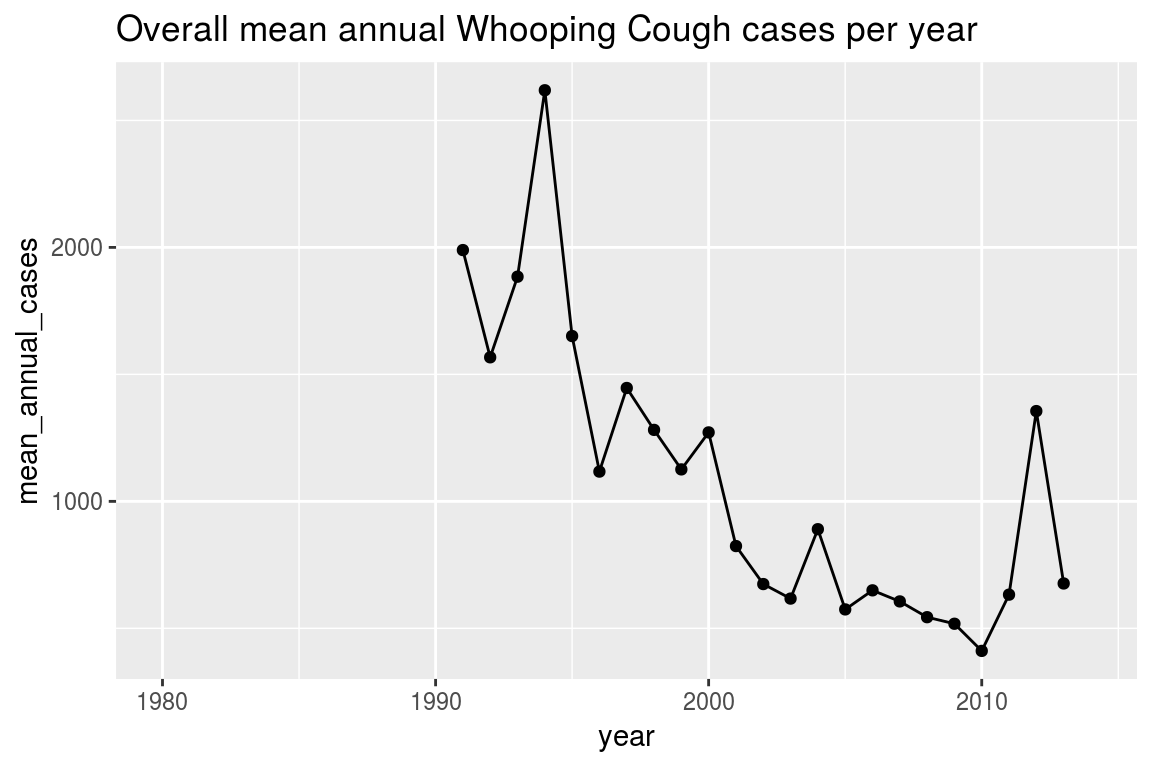
\includegraphics{demo_walkthrough_files/figure-latex/unnamed-chunk-5-1.pdf}

\subsection{Data for individual countries, over
time}\label{data-for-individual-countries-over-time}

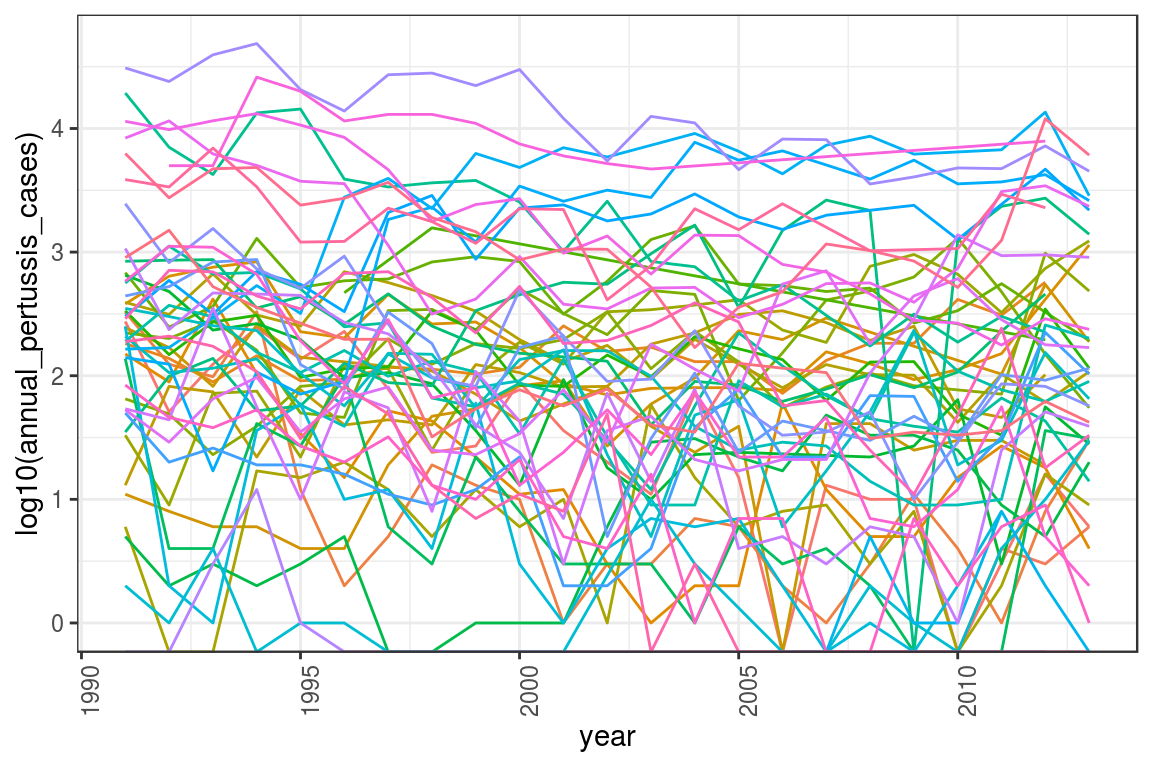
\includegraphics{demo_walkthrough_files/figure-latex/unnamed-chunk-6-1.pdf}

\subsection{Data for only The
Netherlands}\label{data-for-only-the-netherlands}

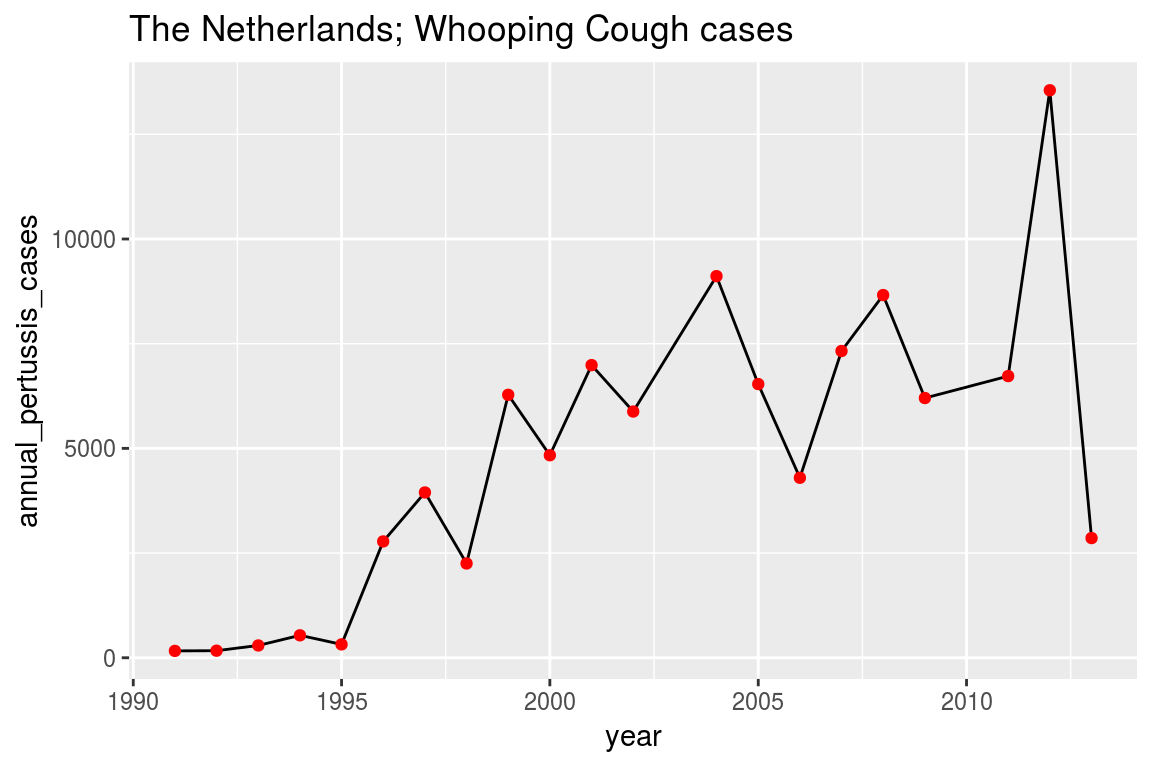
\includegraphics{demo_walkthrough_files/figure-latex/unnamed-chunk-7-1.pdf}

\subsection{Plot linear model for NL}\label{plot-linear-model-for-nl}

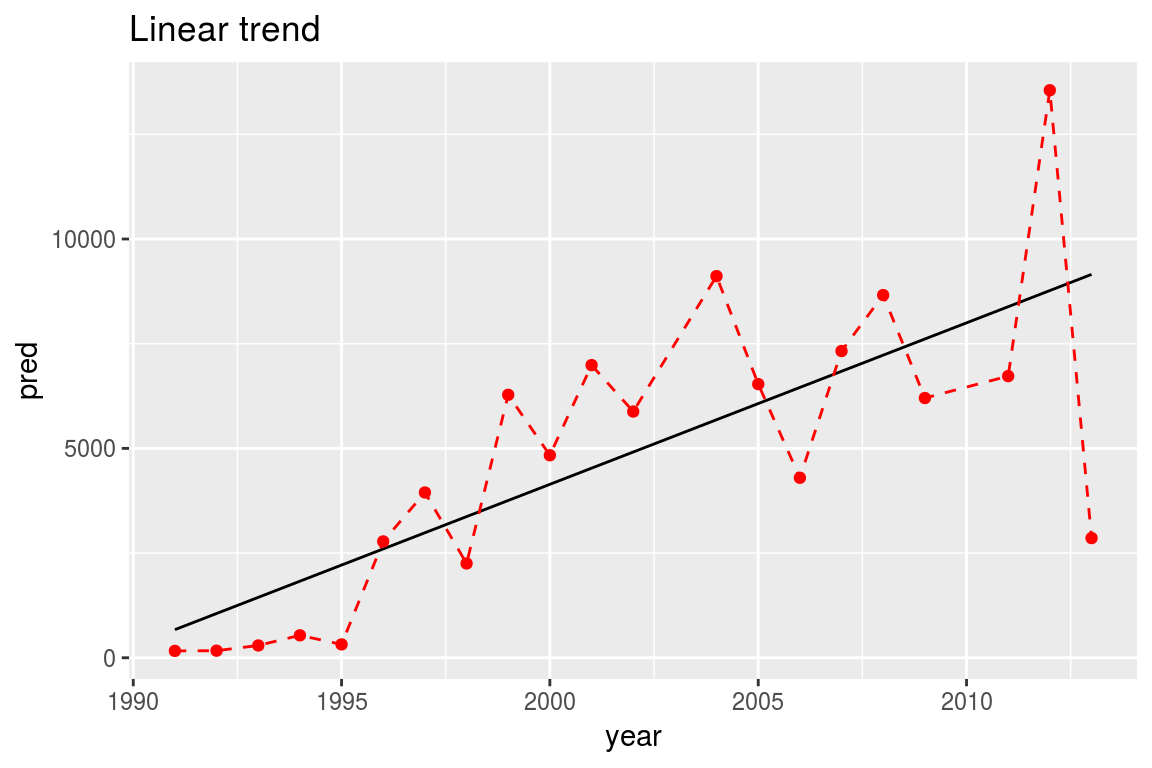
\includegraphics{demo_walkthrough_files/figure-latex/unnamed-chunk-8-1.pdf}

\subsection{\texorpdfstring{How can we apply this to \texttt{every}
country in the
dataset?}{How can we apply this to every country in the dataset?}}\label{how-can-we-apply-this-to-every-country-in-the-dataset}

Without doing the above 53 times

\subsection{Split the data by country and apply the model or graphing
code to each
subset}\label{split-the-data-by-country-and-apply-the-model-or-graphing-code-to-each-subset}

\begin{itemize}
\tightlist
\item
  In fact, data for each country is a subset of the full dataset
\item
  We can subset the original dataframe into seperate dataframes for each
  country
\end{itemize}

\subsection{List-columns to track your results and
models}\label{list-columns-to-track-your-results-and-models}

\begin{Shaded}
\begin{Highlighting}[]
\NormalTok{nested_pertussis <-}\StringTok{ }\NormalTok{pertussis_data_tidy }\OperatorTok
\StringTok{  }\KeywordTok{na.omit}\NormalTok{() }\OperatorTok
\StringTok{  }\NormalTok{dplyr}\OperatorTok{::}\KeywordTok{select}\NormalTok{(country, year, annual_pertussis_cases) }\OperatorTok
\StringTok{  }\KeywordTok{group_by}\NormalTok{(country) }\OperatorTok
\StringTok{    }\KeywordTok{nest}\NormalTok{() }
\end{Highlighting}
\end{Shaded}

\subsection{Inspecting the nested
dataframes}\label{inspecting-the-nested-dataframes}

\begin{Shaded}
\begin{Highlighting}[]
\KeywordTok{head}\NormalTok{(nested_pertussis, }\DecValTok{2}\NormalTok{) ## you see the grouping by country}
\end{Highlighting}
\end{Shaded}

\begin{verbatim}
## # A tibble: 2 x 2
##   country data             
##   <chr>   <list>           
## 1 Albania <tibble [22 x 2]>
## 2 Armenia <tibble [23 x 2]>
\end{verbatim}

\begin{Shaded}
\begin{Highlighting}[]
\KeywordTok{head}\NormalTok{(nested_pertussis}\OperatorTok{$}\NormalTok{data[[}\DecValTok{1}\NormalTok{]], }\DecValTok{2}\NormalTok{) ## you get the individual country df}
\end{Highlighting}
\end{Shaded}

\begin{verbatim}
## # A tibble: 2 x 2
##   year       annual_pertussis_cases
##   <date>                      <int>
## 1 1991-01-01                    275
## 2 1992-01-01                     51
\end{verbatim}

\subsection{Label (name) the idividual elements of the list
column}\label{label-name-the-idividual-elements-of-the-list-column}

\begin{Shaded}
\begin{Highlighting}[]
\KeywordTok{names}\NormalTok{(nested_pertussis}\OperatorTok{$}\NormalTok{data) <-}\StringTok{ }\NormalTok{nested_pertussis}\OperatorTok{$}\NormalTok{country }
\KeywordTok{head}\NormalTok{(nested_pertussis}\OperatorTok{$}\NormalTok{data, }\DecValTok{1}\NormalTok{)}
\end{Highlighting}
\end{Shaded}

\subsection{Linear model for each
country}\label{linear-model-for-each-country}

First we write a function that creates the linear model for one country

\begin{Shaded}
\begin{Highlighting}[]
\NormalTok{country_model_lm <-}\StringTok{ }\ControlFlowTok{function}\NormalTok{(df)\{}
\NormalTok{  model <-}\StringTok{ }\KeywordTok{lm}\NormalTok{(}
\NormalTok{    annual_pertussis_cases }\OperatorTok{~}\StringTok{ }\NormalTok{year, }
    \DataTypeTok{data =}\NormalTok{ df)}
  \KeywordTok{return}\NormalTok{(model)}
\NormalTok{\}}
\end{Highlighting}
\end{Shaded}

\subsection{\texorpdfstring{Iterate the model function over nested
\texttt{\$data} with
\texttt{purrr::map()}}{Iterate the model function over nested \$data with purrr::map()}}\label{iterate-the-model-function-over-nested-data-with-purrrmap}

\begin{Shaded}
\begin{Highlighting}[]
\NormalTok{models <-}\StringTok{ }\KeywordTok{map}\NormalTok{(}
\NormalTok{  nested_pertussis}\OperatorTok{$}\NormalTok{data, country_model_lm}
\NormalTok{  )}
\KeywordTok{head}\NormalTok{(models, }\DecValTok{2}\NormalTok{)}
\end{Highlighting}
\end{Shaded}

\begin{verbatim}
## [[1]]
## 
## Call:
## lm(formula = annual_pertussis_cases ~ year, data = df)
## 
## Coefficients:
## (Intercept)         year  
##   356.23325     -0.02502  
## 
## 
## [[2]]
## 
## Call:
## lm(formula = annual_pertussis_cases ~ year, data = df)
## 
## Coefficients:
## (Intercept)         year  
##   297.70414     -0.02168
\end{verbatim}

\subsection{Keep it togetheR}\label{keep-it-together}

\begin{itemize}
\tightlist
\item
  We have the models now
\item
  Better to store them together with the data and the group (`country')
  info
\item
  By using \texttt{dplyr::mutate()} in conjunction with \texttt{map()}
\end{itemize}

{[}\texttt{map()} vs.
\texttt{lapply()}{]}\url{https://stackoverflow.com/questions/45101045/why-use-purrrmap-instead-of-lapply})

\subsection{Create an additional list-column on the basis of an existing
one}\label{create-an-additional-list-column-on-the-basis-of-an-existing-one}

\begin{Shaded}
\begin{Highlighting}[]
\NormalTok{nested_pertussis <-}\StringTok{ }\NormalTok{nested_pertussis }\OperatorTok
\StringTok{  }\KeywordTok{mutate}\NormalTok{(}\DataTypeTok{models_lm =} \KeywordTok{map}\NormalTok{(data, country_model_lm))}
\KeywordTok{head}\NormalTok{(nested_pertussis, }\DecValTok{2}\NormalTok{)}
\end{Highlighting}
\end{Shaded}

\begin{verbatim}
## # A tibble: 2 x 3
##   country data              models_lm
##   <chr>   <list>            <list>   
## 1 Albania <tibble [22 x 2]> <S3: lm> 
## 2 Armenia <tibble [23 x 2]> <S3: lm>
\end{verbatim}

\subsection{Add model summaries as a
list-column}\label{add-model-summaries-as-a-list-column}

\begin{Shaded}
\begin{Highlighting}[]
\NormalTok{nested_pertussis <-}\StringTok{ }\NormalTok{nested_pertussis }\OperatorTok
\StringTok{  }\KeywordTok{mutate}\NormalTok{(}\DataTypeTok{models_lm_summary =} \KeywordTok{map}\NormalTok{(models_lm, summary))}
\KeywordTok{head}\NormalTok{(nested_pertussis, }\DecValTok{2}\NormalTok{)}
\end{Highlighting}
\end{Shaded}

\begin{verbatim}
## # A tibble: 2 x 4
##   country data              models_lm models_lm_summary
##   <chr>   <list>            <list>    <list>           
## 1 Albania <tibble [22 x 2]> <S3: lm>  <S3: summary.lm> 
## 2 Armenia <tibble [23 x 2]> <S3: lm>  <S3: summary.lm>
\end{verbatim}

\subsection{\texorpdfstring{Extracting information from a list-column of
models; \texttt{glance()} \&
\texttt{pluck()}}{Extracting information from a list-column of models; glance() \& pluck()}}\label{extracting-information-from-a-list-column-of-models-glance-pluck}

\begin{Shaded}
\begin{Highlighting}[]
\NormalTok{nested_pertussis <-}\StringTok{ }\NormalTok{nested_pertussis }\OperatorTok
\StringTok{  }\KeywordTok{mutate}\NormalTok{(}\DataTypeTok{params_lm =}  \KeywordTok{map}\NormalTok{(models_lm, broom}\OperatorTok{::}\NormalTok{glance)) }\OperatorTok
\StringTok{  }\KeywordTok{mutate}\NormalTok{(}\DataTypeTok{p_value =} \KeywordTok{map}\NormalTok{(params_lm, pluck, }\StringTok{"p.value"}\NormalTok{))}

\NormalTok{nested_pertussis}\OperatorTok{$}\NormalTok{params_lm[[}\DecValTok{1}\NormalTok{]]}
\end{Highlighting}
\end{Shaded}

\begin{verbatim}
## # A tibble: 1 x 11
##   r.squared adj.r.squared sigma statistic p.value    df logLik   AIC   BIC
##       <dbl>         <dbl> <dbl>     <dbl>   <dbl> <int>  <dbl> <dbl> <dbl>
## 1     0.529         0.505  58.8      22.4 1.27e-4     2  -120.  246.  249.
## # ... with 2 more variables: deviance <dbl>, df.residual <int>
\end{verbatim}

\begin{Shaded}
\begin{Highlighting}[]
\NormalTok{nested_pertussis}\OperatorTok{$}\NormalTok{p_value[[}\DecValTok{1}\NormalTok{]] }\OperatorTok\StringTok{ }\KeywordTok{round}\NormalTok{(}\DecValTok{6}\NormalTok{)}
\end{Highlighting}
\end{Shaded}

\begin{verbatim}
## [1] 0.000127
\end{verbatim}

\subsection{Adding a list of plots in a
column}\label{adding-a-list-of-plots-in-a-column}

A function that creates a graph for a single country

\begin{Shaded}
\begin{Highlighting}[]
\NormalTok{plot_line <-}\StringTok{ }\ControlFlowTok{function}\NormalTok{(df, key)\{}
  
\NormalTok{  model <-}\StringTok{ }\KeywordTok{lm}\NormalTok{(}
\NormalTok{  annual_pertussis_cases }\OperatorTok{~}\StringTok{ }\NormalTok{year, }
  \DataTypeTok{data =}\NormalTok{ df }\OperatorTok
\StringTok{    }\KeywordTok{na.omit}\NormalTok{()}
\NormalTok{)}
\NormalTok{## plot model for NL}

\NormalTok{plot <-}\StringTok{ }\NormalTok{df }\OperatorTok
\StringTok{  }\KeywordTok{na.omit}\NormalTok{() }\OperatorTok
\StringTok{  }\KeywordTok{add_predictions}\NormalTok{(model) }\OperatorTok
\StringTok{  }\KeywordTok{ggplot}\NormalTok{(}\KeywordTok{aes}\NormalTok{(}\DataTypeTok{x =}\NormalTok{ year, }
             \DataTypeTok{y =}\NormalTok{ pred)) }\OperatorTok{+}
\StringTok{  }\KeywordTok{geom_line}\NormalTok{() }\OperatorTok{+}
\StringTok{  }\KeywordTok{geom_point}\NormalTok{(}
    \DataTypeTok{data =}\NormalTok{ df,}
    \KeywordTok{aes}\NormalTok{(}\DataTypeTok{x =}\NormalTok{ year, }
    \DataTypeTok{y =}\NormalTok{ annual_pertussis_cases),}
    \DataTypeTok{colour =} \StringTok{"red"}\NormalTok{) }\OperatorTok{+}
\StringTok{  }\KeywordTok{geom_line}\NormalTok{(}
    \DataTypeTok{data =}\NormalTok{ df }\OperatorTok\StringTok{ }\NormalTok{na.omit, ## note the pipe to remove NA}
    \KeywordTok{aes}\NormalTok{(}\DataTypeTok{x =}\NormalTok{ year, }
        \DataTypeTok{y =}\NormalTok{ annual_pertussis_cases),}
    \DataTypeTok{colour =} \StringTok{"red"}\NormalTok{,}
    \DataTypeTok{linetype =} \StringTok{"dashed"}
\NormalTok{) }\OperatorTok{+}
\StringTok{  }\KeywordTok{ggtitle}\NormalTok{(}\KeywordTok{paste}\NormalTok{(}\StringTok{"Linear model for"}\NormalTok{, key }\OperatorTok\StringTok{ }\KeywordTok{as.character}\NormalTok{()))}

  \KeywordTok{return}\NormalTok{(plot)}
\NormalTok{\}}
\end{Highlighting}
\end{Shaded}

\subsection{Iterate plot function over nested
data}\label{iterate-plot-function-over-nested-data}

\begin{Shaded}
\begin{Highlighting}[]
\NormalTok{nested_pertussis <-}\StringTok{ }\NormalTok{nested_pertussis }\OperatorTok\StringTok{ }
\StringTok{  }\KeywordTok{mutate}\NormalTok{(}
    \DataTypeTok{plots_lm =} \KeywordTok{map2}\NormalTok{(data, country, plot_line)}
\NormalTok{  )}
\NormalTok{nested_pertussis}
\end{Highlighting}
\end{Shaded}

\begin{verbatim}
## # A tibble: 52 x 7
##    country   data    models_lm models_lm_summa~ params_lm  p_value plots_lm
##    <chr>     <list>  <list>    <list>           <list>     <list>  <list>  
##  1 Albania   <tibbl~ <S3: lm>  <S3: summary.lm> <tibble [~ <dbl [~ <S3: gg>
##  2 Armenia   <tibbl~ <S3: lm>  <S3: summary.lm> <tibble [~ <dbl [~ <S3: gg>
##  3 Austria   <tibbl~ <S3: lm>  <S3: summary.lm> <tibble [~ <dbl [~ <S3: gg>
##  4 Azerbaij~ <tibbl~ <S3: lm>  <S3: summary.lm> <tibble [~ <dbl [~ <S3: gg>
##  5 Belarus   <tibbl~ <S3: lm>  <S3: summary.lm> <tibble [~ <dbl [~ <S3: gg>
##  6 Belgium   <tibbl~ <S3: lm>  <S3: summary.lm> <tibble [~ <dbl [~ <S3: gg>
##  7 Bosnia a~ <tibbl~ <S3: lm>  <S3: summary.lm> <tibble [~ <dbl [~ <S3: gg>
##  8 Bulgaria  <tibbl~ <S3: lm>  <S3: summary.lm> <tibble [~ <dbl [~ <S3: gg>
##  9 Croatia   <tibbl~ <S3: lm>  <S3: summary.lm> <tibble [~ <dbl [~ <S3: gg>
## 10 Cyprus    <tibbl~ <S3: lm>  <S3: summary.lm> <tibble [~ <dbl [~ <S3: gg>
## # ... with 42 more rows
\end{verbatim}

\subsection{Name elements in the
list-column}\label{name-elements-in-the-list-column}

\begin{Shaded}
\begin{Highlighting}[]
\KeywordTok{names}\NormalTok{(nested_pertussis}\OperatorTok{$}\NormalTok{plots_lm) <-}\StringTok{ }\NormalTok{nested_pertussis}\OperatorTok{$}\NormalTok{country}
\end{Highlighting}
\end{Shaded}

\subsection{Show a plot}\label{show-a-plot}

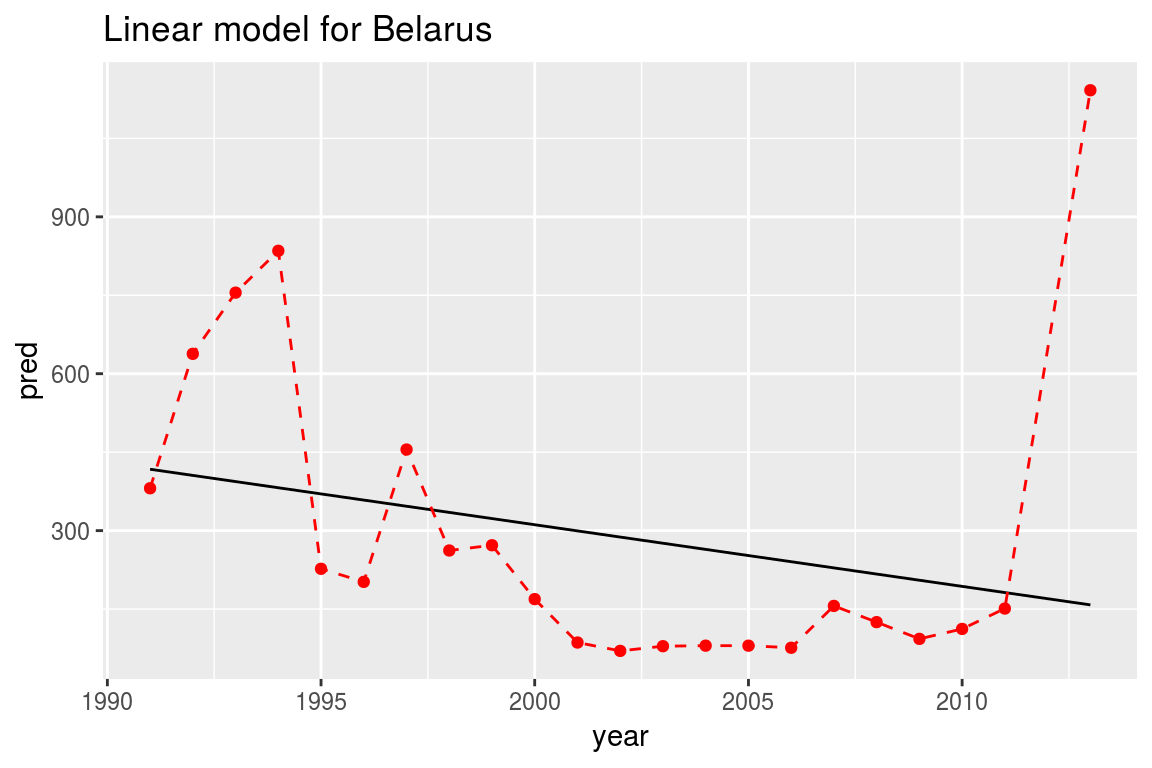
\includegraphics{demo_walkthrough_files/figure-latex/unnamed-chunk-20-1.pdf}

\subsection{Panel of plots}\label{panel-of-plots}

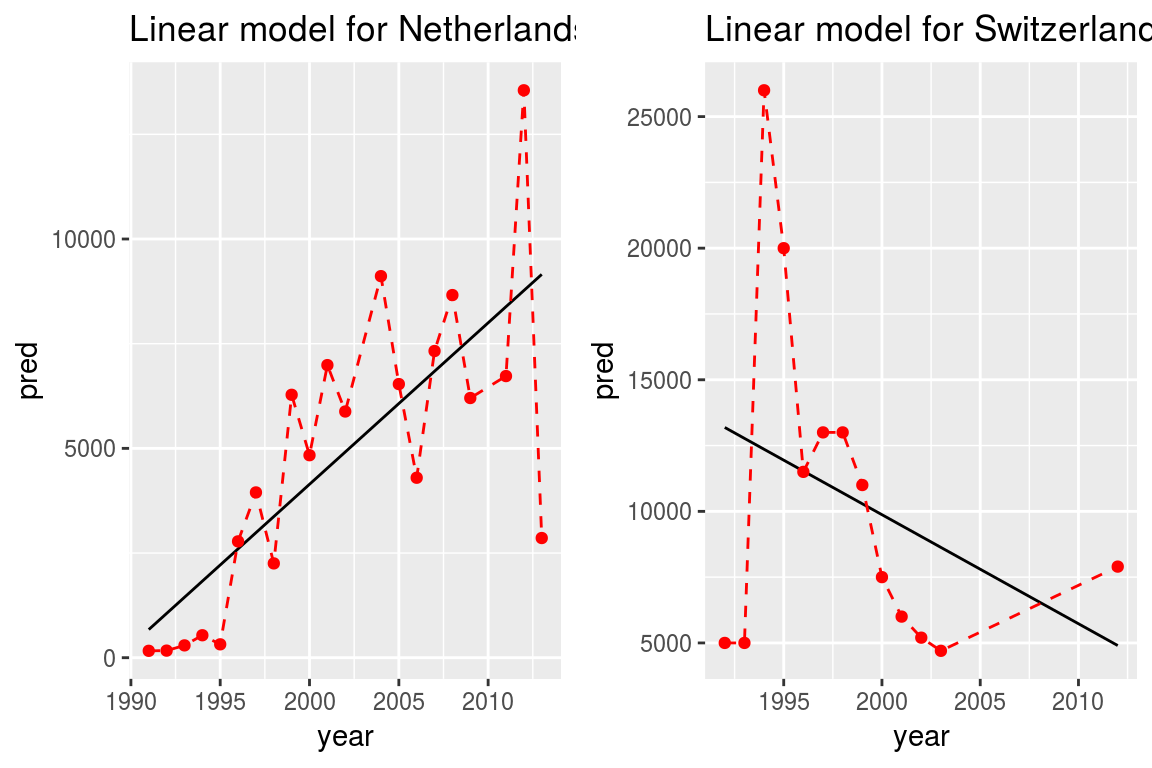
\includegraphics{demo_walkthrough_files/figure-latex/unnamed-chunk-21-1.pdf}

\subsection{Consider this}\label{consider-this}

Imagine you are writing/using a function to loop over data or models in
a list-(column) with \texttt{map()} or \texttt{lapply}, but it throws an
ERROR half way through the list, stopping the loop

How would you solve this?

The answer is PART II below

\subsection{Learn more?}\label{learn-more}

`Managing many models with R' by Hadley Wickham - Lecture
\url{https://www.youtube.com/watch?v=rz3_FDVt9eg}

`R for Data Science' by Garret Grolemund \& Hadley Wickham
\url{https://r4ds.had.co.nz/} Especially chapters: 21 -
\url{https://r4ds.had.co.nz/iteration.html} 25 -
\url{https://r4ds.had.co.nz/many-models.html}

\subsection{}\label{section-1}

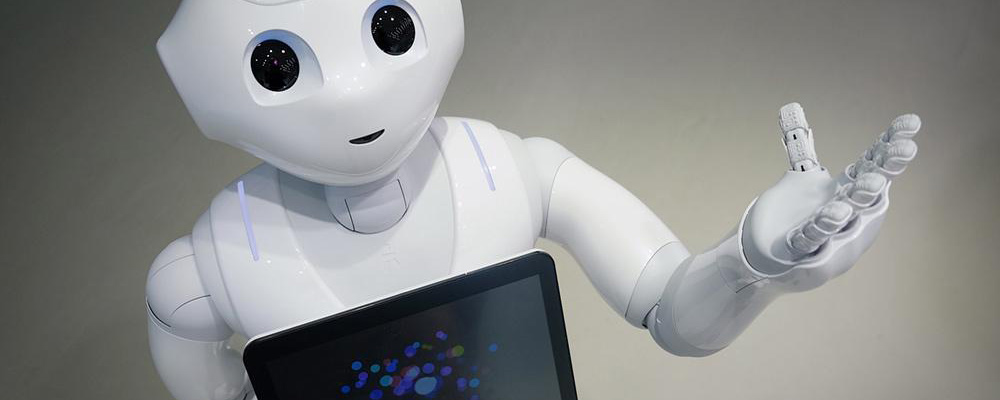
\includegraphics{/home/marc_teunis/rcafe/images/pepper.jpg}

\section{PART II; Extracting more information from a list
column}\label{part-ii-extracting-more-information-from-a-list-column}

\textbf{ADVANCED}

For another day\ldots{}

\subsection{Looking at quantative statistical measures for model
quality}\label{looking-at-quantative-statistical-measures-for-model-quality}

\begin{Shaded}
\begin{Highlighting}[]
\NormalTok{r_squared <-}\StringTok{ }\NormalTok{nested_pertussis }\OperatorTok
\StringTok{  }\NormalTok{dplyr}\OperatorTok{::}\KeywordTok{filter}\NormalTok{(country }\OperatorTok{!=}\StringTok{ "Monaco"}\NormalTok{) }\OperatorTok\StringTok{ }\NormalTok{## remove Monaco (incomplete data)}
\StringTok{  }\KeywordTok{mutate}\NormalTok{(}\DataTypeTok{glance =} \KeywordTok{map}\NormalTok{(models_lm, broom}\OperatorTok{::}\NormalTok{glance)) }\OperatorTok\StringTok{ }
\StringTok{  }\KeywordTok{unnest}\NormalTok{(glance, }\DataTypeTok{drop =} \OtherTok{TRUE}\NormalTok{) }\OperatorTok
\StringTok{  }\KeywordTok{select}\NormalTok{(country, r.squared, AIC, BIC) }\OperatorTok
\StringTok{  }\KeywordTok{arrange}\NormalTok{(r.squared)}
\end{Highlighting}
\end{Shaded}

\subsection{Plotting r.sqared values}\label{plotting-r.sqared-values}

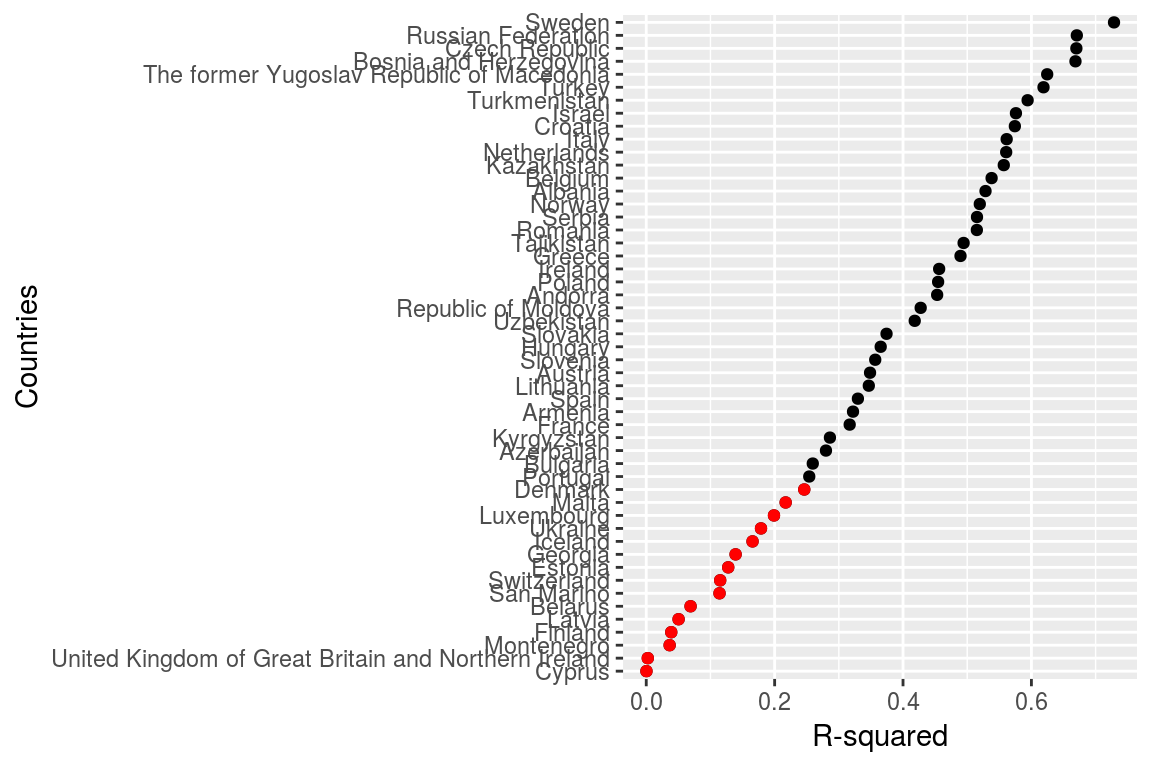
\includegraphics{demo_walkthrough_files/figure-latex/unnamed-chunk-24-1.pdf}

\subsection{Plotting pertussis cases for countries with low r.squared
over
time}\label{plotting-pertussis-cases-for-countries-with-low-r.squared-over-time}

\begin{enumerate}
\def\labelenumi{\arabic{enumi}.}
\tightlist
\item
  Filter countries with \texttt{r.squared} \textless{}= 0.25
\item
  Put countries in vector
\item
  Plot data
\end{enumerate}

\subsection{Step 1}\label{step-1}

\begin{Shaded}
\begin{Highlighting}[]
\NormalTok{low_r_squared <-}\StringTok{ }\NormalTok{r_squared }\OperatorTok
\StringTok{  }\NormalTok{dplyr}\OperatorTok{::}\KeywordTok{filter}\NormalTok{(r.squared }\OperatorTok{<=}\StringTok{ }\FloatTok{0.25}\NormalTok{) }\OperatorTok
\StringTok{  }\NormalTok{dplyr}\OperatorTok{::}\KeywordTok{select}\NormalTok{(country) }
\NormalTok{low_r_squared <-}\StringTok{ }\NormalTok{low_r_squared}\OperatorTok{$}\NormalTok{country}
\end{Highlighting}
\end{Shaded}

\subsection{Step 2}\label{step-2}

\begin{Shaded}
\begin{Highlighting}[]
\NormalTok{low_r_squared_nested <-}\StringTok{ }\NormalTok{nested_pertussis }\OperatorTok
\StringTok{  }\NormalTok{dplyr}\OperatorTok{::}\KeywordTok{filter}\NormalTok{(country }\OperatorTok\StringTok{ }\NormalTok{low_r_squared) }\OperatorTok
\StringTok{  }\KeywordTok{select}\NormalTok{(country, data) }\OperatorTok
\StringTok{  }\KeywordTok{unnest}\NormalTok{()}
\end{Highlighting}
\end{Shaded}

\subsection{Step 3}\label{step-3}

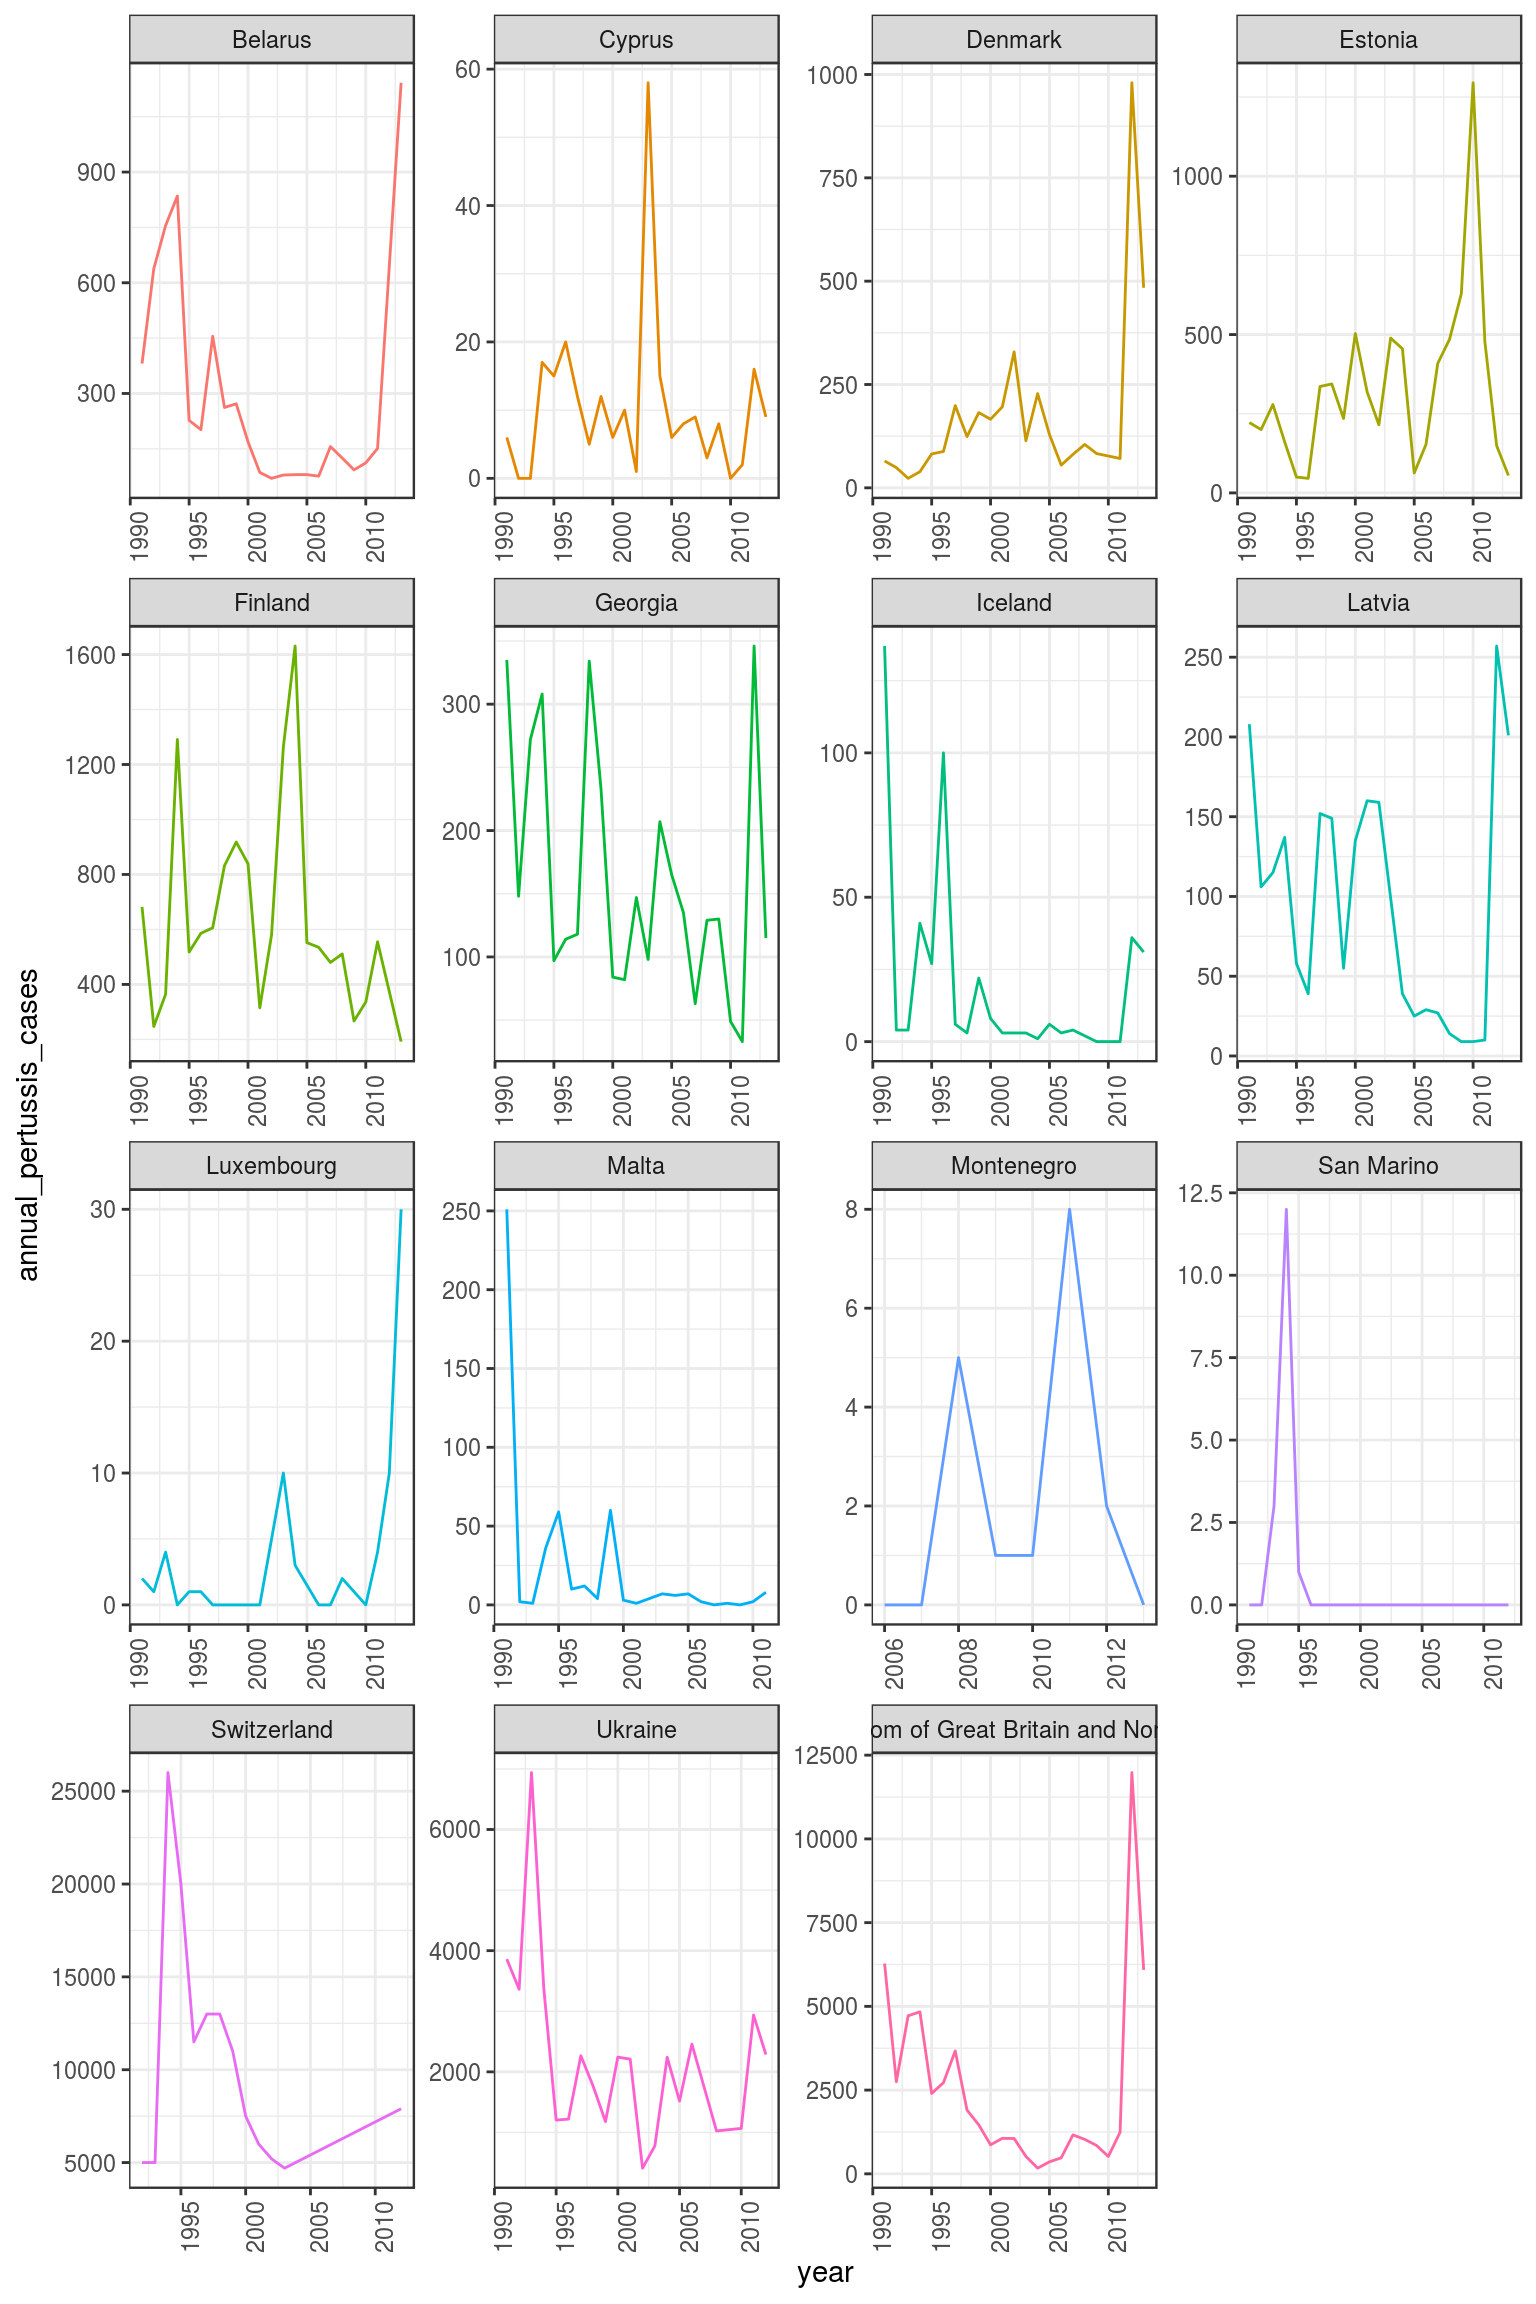
\includegraphics{demo_walkthrough_files/figure-latex/unnamed-chunk-27-1.pdf}

What is happening to the pertussis vaccination grade over the past 8
years?

\subsection{Store ggplot2 objects in a
list-column}\label{store-ggplot2-objects-in-a-list-column}

\begin{enumerate}
\def\labelenumi{\arabic{enumi}.}
\tightlist
\item
  Create a function that makes the plot
\item
  Test function on single dataframe
\item
  Apply the function using \texttt{mutate()} and \texttt{map()} to all
  dataframes or models
\end{enumerate}

\begin{Shaded}
\begin{Highlighting}[]
\NormalTok{## isolate one dataframe to test function}
\NormalTok{df <-}\StringTok{ }\NormalTok{nested_pertussis}\OperatorTok{$}\NormalTok{data[[}\DecValTok{1}\NormalTok{]]}
\NormalTok{plot_country <-}\StringTok{ }\ControlFlowTok{function}\NormalTok{(df)\{}
  
\NormalTok{  df }\OperatorTok
\StringTok{    }\KeywordTok{ggplot}\NormalTok{(}\KeywordTok{aes}\NormalTok{(}\DataTypeTok{x =}\NormalTok{ year,}
           \DataTypeTok{y =}\NormalTok{ annual_pertussis_cases)) }\OperatorTok{+}
\StringTok{    }\KeywordTok{geom_line}\NormalTok{() }\OperatorTok{+}
\StringTok{    }\KeywordTok{geom_smooth}\NormalTok{() }\OperatorTok{+}
\StringTok{    }\KeywordTok{ylab}\NormalTok{(}\StringTok{"Annual cases"}\NormalTok{)}

\NormalTok{\}}

\NormalTok{## test function}
\CommentTok{# plot_country(df = df)}
\end{Highlighting}
\end{Shaded}

\subsection{Apply plotting function to nested
data}\label{apply-plotting-function-to-nested-data}

\begin{Shaded}
\begin{Highlighting}[]
\NormalTok{nested_pertussis <-}\StringTok{ }\NormalTok{nested_pertussis }\OperatorTok
\StringTok{  }\KeywordTok{mutate}\NormalTok{(}\DataTypeTok{plots_cases_over_time =} \KeywordTok{map}\NormalTok{(data, }
\NormalTok{                                     plot_country))}
\end{Highlighting}
\end{Shaded}

\subsection{Add countries as names to
nest-column}\label{add-countries-as-names-to-nest-column}

\begin{Shaded}
\begin{Highlighting}[]
\KeywordTok{names}\NormalTok{(nested_pertussis}\OperatorTok{$}\NormalTok{plots_cases_over_time) <-}\StringTok{ }
\StringTok{  }\KeywordTok{c}\NormalTok{(nested_pertussis}\OperatorTok{$}\NormalTok{country)}

\NormalTok{nested_pertussis}\OperatorTok{$}\NormalTok{plots_cases_over_time[}\DecValTok{1}\NormalTok{]}
\end{Highlighting}
\end{Shaded}

\begin{verbatim}
## $Albania
\end{verbatim}

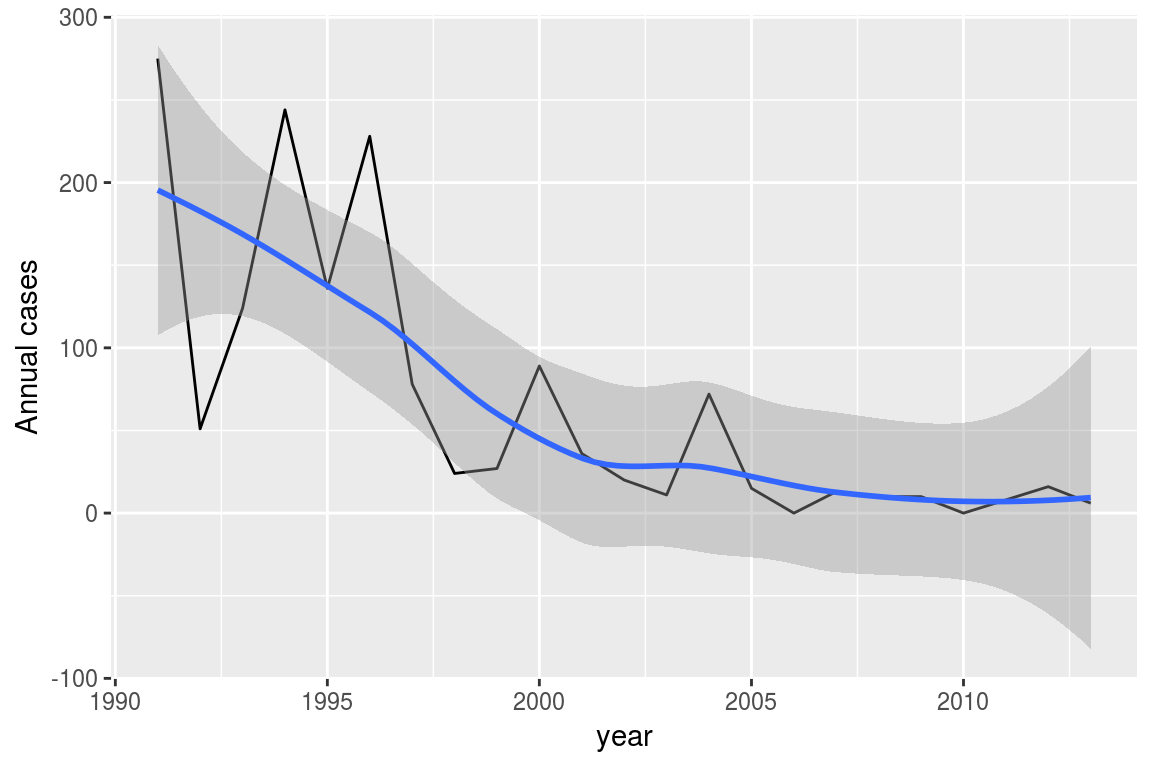
\includegraphics{demo_walkthrough_files/figure-latex/unnamed-chunk-30-1.pdf}

\subsection{\texorpdfstring{Pull out ``The
Netherlands''}{Pull out The Netherlands}}\label{pull-out-the-netherlands}

\begin{Shaded}
\begin{Highlighting}[]
\NormalTok{nested_pertussis}\OperatorTok{$}\NormalTok{plots_cases_over_time}\OperatorTok{$}\NormalTok{Netherlands}
\end{Highlighting}
\end{Shaded}

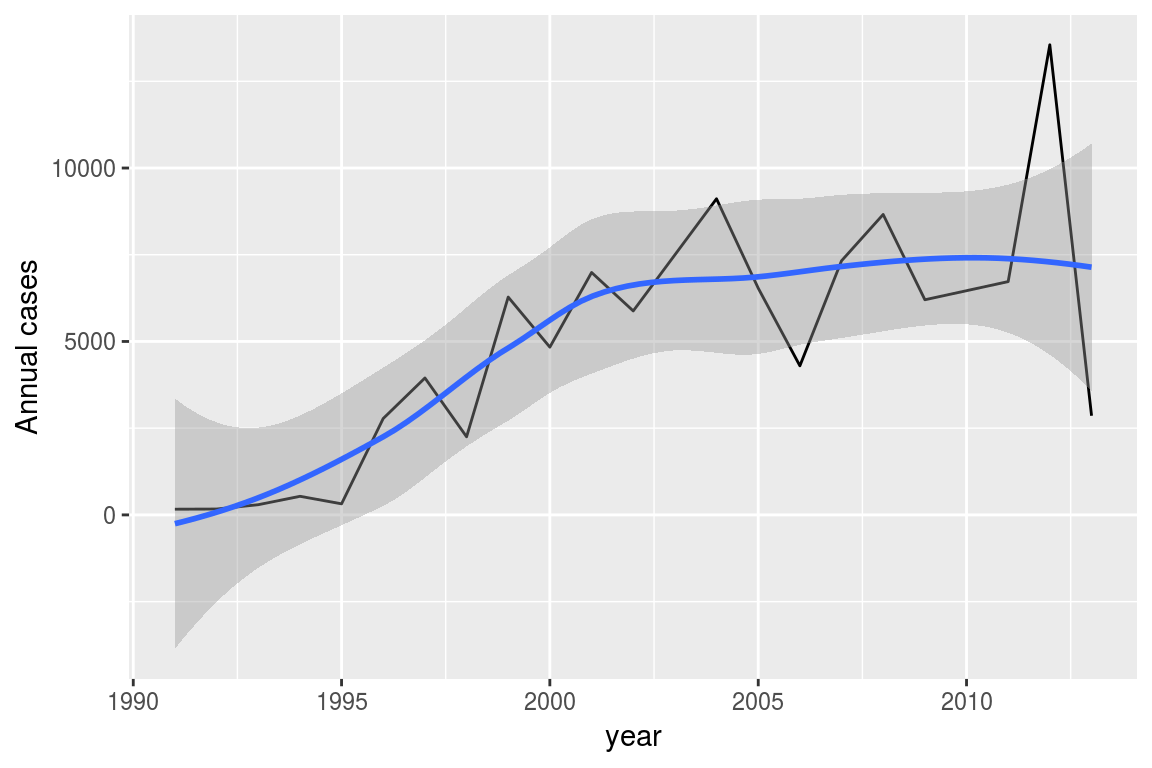
\includegraphics{demo_walkthrough_files/figure-latex/unnamed-chunk-31-1.pdf}

\subsection{Plotting a panel of 4
graphs}\label{plotting-a-panel-of-4-graphs}

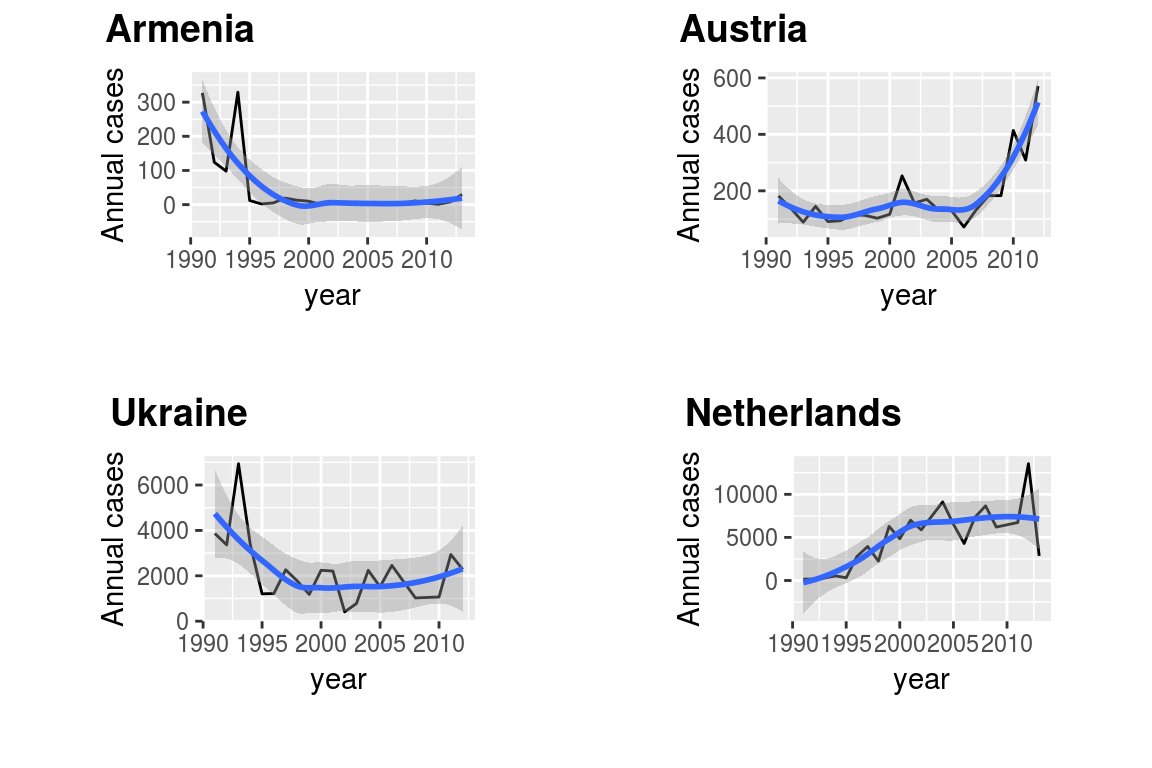
\includegraphics{demo_walkthrough_files/figure-latex/unnamed-chunk-32-1.pdf}

\subsection{Literature}\label{literature}

For some background on the pattern we are seeing

\begin{itemize}
\tightlist
\item
  \url{https://www.scientificamerican.com/article/why-whooping-cough-vaccines-are-wearing-off/}
\item
  \url{http://outbreaknewstoday.com/pertussis-cases-up-significantly-in-the-eu-netherlands-and-uk-worst-hit-55315/}
\end{itemize}

\subsection{Exploring many more
models}\label{exploring-many-more-models}

Let's add a quadratic model in the mix. Assume we want to explore
non-linear relationships in this dataset

\begin{Shaded}
\begin{Highlighting}[]
\NormalTok{non_linear_model <-}\StringTok{ }\ControlFlowTok{function}\NormalTok{(df, model_params)\{}
  
\NormalTok{  nl_model <-}\StringTok{ }\KeywordTok{lm}\NormalTok{(}
\NormalTok{    annual_pertussis_cases }\OperatorTok{~}\StringTok{ }\KeywordTok{poly}\NormalTok{(year, }
\NormalTok{                                  model_params),}
                 \DataTypeTok{data =}\NormalTok{ df)}
  
  \KeywordTok{return}\NormalTok{(nl_model)}
\NormalTok{\}}
\end{Highlighting}
\end{Shaded}

\subsection{Creating a safe version of this
function}\label{creating-a-safe-version-of-this-function}

\begin{Shaded}
\begin{Highlighting}[]
\NormalTok{safe_non_linear <-}\StringTok{ }\NormalTok{purrr}\OperatorTok{::}\KeywordTok{safely}\NormalTok{(non_linear_model)}
\NormalTok{## apply test:}
\NormalTok{df =}\StringTok{ }\NormalTok{nested_pertussis}\OperatorTok{$}\NormalTok{data[[}\DecValTok{1}\NormalTok{]]}

\NormalTok{test_non_linear <-}\StringTok{  }\NormalTok{df }\OperatorTok\StringTok{ }\KeywordTok{non_linear_model}\NormalTok{(}\DataTypeTok{df =}\NormalTok{ .,}
                                            \DataTypeTok{model_params =} \DecValTok{2}\NormalTok{)}
\end{Highlighting}
\end{Shaded}

\subsection{Test function on one
country}\label{test-function-on-one-country}

\begin{Shaded}
\begin{Highlighting}[]
\NormalTok{test_non_linear }\OperatorTok\StringTok{ }\NormalTok{broom}\OperatorTok{::}\KeywordTok{glance}\NormalTok{()}
\end{Highlighting}
\end{Shaded}

\begin{verbatim}
## # A tibble: 1 x 11
##   r.squared adj.r.squared sigma statistic p.value    df logLik   AIC   BIC
##       <dbl>         <dbl> <dbl>     <dbl>   <dbl> <int>  <dbl> <dbl> <dbl>
## 1     0.607         0.566  55.0      14.7 1.39e-4     3  -118.  244.  248.
## # ... with 2 more variables: deviance <dbl>, df.residual <int>
\end{verbatim}

\subsection{Apply model to all
countries}\label{apply-model-to-all-countries}

We rerun the steps above to add this new model and new graphs to the
nested dataframe

Add new model to the nested table

\begin{Shaded}
\begin{Highlighting}[]
\NormalTok{nested_pertussis <-}\StringTok{ }\NormalTok{nested_pertussis }\OperatorTok
\StringTok{  }\KeywordTok{mutate}\NormalTok{(}\DataTypeTok{models_nl_2 =} \KeywordTok{map}\NormalTok{(data, safe_non_linear, }
                          \DataTypeTok{model_params =} \DecValTok{2}\NormalTok{))}
  
\NormalTok{nested_pertussis}\OperatorTok{$}\NormalTok{models_nl_}\DecValTok{2}\NormalTok{ <-}\StringTok{ }\KeywordTok{transpose}\NormalTok{(nested_pertussis}\OperatorTok{$}\NormalTok{models_nl_}\DecValTok{2}\NormalTok{)}
\end{Highlighting}
\end{Shaded}

\subsection{Set names to elements in the
list-column}\label{set-names-to-elements-in-the-list-column}

To be able to \texttt{pluck()} by name later

\begin{Shaded}
\begin{Highlighting}[]
\KeywordTok{names}\NormalTok{(nested_pertussis}\OperatorTok{$}\NormalTok{models_nl_}\DecValTok{2}\OperatorTok{$}\NormalTok{result) <-}\StringTok{ }\NormalTok{nested_pertussis}\OperatorTok{$}\NormalTok{country}
\end{Highlighting}
\end{Shaded}

\subsection{Pluck results in new
list-column}\label{pluck-results-in-new-list-column}

\begin{Shaded}
\begin{Highlighting}[]
\NormalTok{nested_pertussis}\OperatorTok{$}\NormalTok{models_nl_}\DecValTok{2}\OperatorTok{$}\NormalTok{result[[}\DecValTok{1}\NormalTok{]] }\OperatorTok\StringTok{ }\NormalTok{summary}
\end{Highlighting}
\end{Shaded}

\begin{verbatim}
## 
## Call:
## lm(formula = annual_pertussis_cases ~ poly(year, model_params), 
##     data = df)
## 
## Residuals:
##      Min       1Q   Median       3Q      Max 
## -135.782  -19.621   -3.885    7.188  114.303 
## 
## Coefficients:
##                           Estimate Std. Error t value Pr(>|t|)    
## (Intercept)                  67.50      11.73   5.753 1.52e-05 ***
## poly(year, model_params)1  -278.33      55.03  -5.057 7.00e-05 ***
## poly(year, model_params)2   107.53      55.03   1.954   0.0656 .  
## ---
## Signif. codes:  0 '***' 0.001 '**' 0.01 '*' 0.05 '.' 0.1 ' ' 1
## 
## Residual standard error: 55.03 on 19 degrees of freedom
## Multiple R-squared:  0.6074, Adjusted R-squared:  0.5661 
## F-statistic:  14.7 on 2 and 19 DF,  p-value: 0.0001389
\end{verbatim}

\begin{Shaded}
\begin{Highlighting}[]
\NormalTok{nested_pertussis <-}\StringTok{ }\NormalTok{nested_pertussis }\OperatorTok
\StringTok{  }\KeywordTok{mutate}\NormalTok{(}\DataTypeTok{statistics_nl =} \KeywordTok{pluck}\NormalTok{(models_nl_}\DecValTok{2}\NormalTok{, }\StringTok{"result"}\NormalTok{))}

\NormalTok{nested_pertussis}\OperatorTok{$}\NormalTok{statistics_nl[[}\DecValTok{1}\NormalTok{]] }\OperatorTok\StringTok{ }\NormalTok{summary}
\end{Highlighting}
\end{Shaded}

\begin{verbatim}
## 
## Call:
## lm(formula = annual_pertussis_cases ~ poly(year, model_params), 
##     data = df)
## 
## Residuals:
##      Min       1Q   Median       3Q      Max 
## -135.782  -19.621   -3.885    7.188  114.303 
## 
## Coefficients:
##                           Estimate Std. Error t value Pr(>|t|)    
## (Intercept)                  67.50      11.73   5.753 1.52e-05 ***
## poly(year, model_params)1  -278.33      55.03  -5.057 7.00e-05 ***
## poly(year, model_params)2   107.53      55.03   1.954   0.0656 .  
## ---
## Signif. codes:  0 '***' 0.001 '**' 0.01 '*' 0.05 '.' 0.1 ' ' 1
## 
## Residual standard error: 55.03 on 19 degrees of freedom
## Multiple R-squared:  0.6074, Adjusted R-squared:  0.5661 
## F-statistic:  14.7 on 2 and 19 DF,  p-value: 0.0001389
\end{verbatim}

\subsection{\texorpdfstring{Tidy the list-column with
\texttt{\{broom\}}}{Tidy the list-column with \{broom\}}}\label{tidy-the-list-column-with-broom}

\begin{Shaded}
\begin{Highlighting}[]
\NormalTok{nested_pertussis <-}\StringTok{ }\NormalTok{nested_pertussis }\OperatorTok
\StringTok{  }\KeywordTok{mutate}\NormalTok{(}\DataTypeTok{parameters_nl =} \KeywordTok{map}\NormalTok{(statistics_nl, glance))}
\end{Highlighting}
\end{Shaded}

\subsection{Looking at quantative statistical measures for model
quality}\label{looking-at-quantative-statistical-measures-for-model-quality-1}

\begin{Shaded}
\begin{Highlighting}[]
\NormalTok{r_squared_nl <-}\StringTok{ }\NormalTok{nested_pertussis }\OperatorTok
\StringTok{  }\KeywordTok{select}\NormalTok{(country, parameters_nl) }\OperatorTok
\StringTok{  }\KeywordTok{unnest}\NormalTok{()}
\end{Highlighting}
\end{Shaded}

\subsection{Plotting r.sqared values}\label{plotting-r.sqared-values-1}

\includegraphics{demo_walkthrough_files/figure-latex/unnamed-chunk-41-1.pdf}

\subsection{Let's examine two models for two countries where the
non-linear did and did not not improve the R.squared: Ireland (improved)
and Belgium
(not-improved)}\label{lets-examine-two-models-for-two-countries-where-the-non-linear-did-and-did-not-not-improve-the-r.squared-ireland-improved-and-belgium-not-improved}

\begin{Shaded}
\begin{Highlighting}[]
\NormalTok{x <-}\StringTok{ }\NormalTok{nested_pertussis }\OperatorTok
\StringTok{  }\KeywordTok{select}\NormalTok{(country,}
\NormalTok{         data, }
\NormalTok{         models_lm,}
\NormalTok{         statistics_nl) }\OperatorTok
\StringTok{  }\KeywordTok{gather}\NormalTok{(models_lm}\OperatorTok{:}\NormalTok{statistics_nl, }\DataTypeTok{key =} \StringTok{"models"}\NormalTok{, }\DataTypeTok{value =} \StringTok{"model_params"}\NormalTok{) }\OperatorTok
\StringTok{ }\KeywordTok{print}\NormalTok{()  }
\end{Highlighting}
\end{Shaded}

\begin{verbatim}
## # A tibble: 104 x 4
##    country                data              models    model_params
##    <chr>                  <list>            <chr>     <list>      
##  1 Albania                <tibble [22 x 2]> models_lm <S3: lm>    
##  2 Armenia                <tibble [23 x 2]> models_lm <S3: lm>    
##  3 Austria                <tibble [22 x 2]> models_lm <S3: lm>    
##  4 Azerbaijan             <tibble [23 x 2]> models_lm <S3: lm>    
##  5 Belarus                <tibble [22 x 2]> models_lm <S3: lm>    
##  6 Belgium                <tibble [21 x 2]> models_lm <S3: lm>    
##  7 Bosnia and Herzegovina <tibble [19 x 2]> models_lm <S3: lm>    
##  8 Bulgaria               <tibble [22 x 2]> models_lm <S3: lm>    
##  9 Croatia                <tibble [23 x 2]> models_lm <S3: lm>    
## 10 Cyprus                 <tibble [23 x 2]> models_lm <S3: lm>    
## # ... with 94 more rows
\end{verbatim}

\subsection{\texorpdfstring{Remove `empty
model'}{Remove empty model}}\label{remove-empty-model}

\begin{Shaded}
\begin{Highlighting}[]
\NormalTok{ind <-}\StringTok{ }\NormalTok{x}\OperatorTok{$}\NormalTok{model_params }\OperatorTok{==}\StringTok{ "NULL"}
\CommentTok{#ind <- x$data == "NULL"}
\NormalTok{x <-}\StringTok{ }\NormalTok{x[}\OperatorTok{!}\NormalTok{ind, ]}
\end{Highlighting}
\end{Shaded}

\subsection{Add prediction-list
column}\label{add-prediction-list-column}

\begin{Shaded}
\begin{Highlighting}[]
\NormalTok{predictions <-}\StringTok{ }\NormalTok{x }\OperatorTok
\CommentTok{#  filter(country == "Czech Republic") %>%}
\StringTok{  }\KeywordTok{mutate}\NormalTok{(}\DataTypeTok{predictions =} \KeywordTok{map2}\NormalTok{(data, model_params, add_predictions,}
         \DataTypeTok{var =} \StringTok{"annual_pertussis_cases"}\NormalTok{)) }\OperatorTok
\StringTok{  }\KeywordTok{filter}\NormalTok{(country }\OperatorTok{==}\StringTok{ "Ireland"} \OperatorTok{|}\StringTok{ }
\StringTok{         }\NormalTok{country }\OperatorTok{==}\StringTok{ "Belgium"}\NormalTok{) }\OperatorTok
\StringTok{  }\KeywordTok{select}\NormalTok{(country, data, predictions)}
\end{Highlighting}
\end{Shaded}

\subsection{Set names}\label{set-names}

\begin{Shaded}
\begin{Highlighting}[]
\KeywordTok{names}\NormalTok{(predictions}\OperatorTok{$}\NormalTok{predictions) <-}\StringTok{ }\NormalTok{predictions}\OperatorTok{$}\NormalTok{country}
\end{Highlighting}
\end{Shaded}

\subsection{Belgium}\label{belgium}

\includegraphics{demo_walkthrough_files/figure-latex/unnamed-chunk-46-1.pdf}

\subsection{Ireland}\label{ireland}

\includegraphics{demo_walkthrough_files/figure-latex/unnamed-chunk-47-1.pdf}

\subsection{Learn more?}\label{learn-more-1}

To practice with more examples have a look at

\begin{Shaded}
\begin{Highlighting}[]
\KeywordTok{source}\NormalTok{(}\DataTypeTok{file =} \KeywordTok{file.path}\NormalTok{(root, }\StringTok{"R"}\NormalTok{, }\StringTok{"render_help.R"}\NormalTok{))}
\KeywordTok{help_console}\NormalTok{(}\DataTypeTok{topic =} \StringTok{"repurrrsive"}\NormalTok{)}
\end{Highlighting}
\end{Shaded}

\begin{verbatim}
## _r_e_p_u_r_r_r_s_i_v_e: _E_x_a_m_p_l_e_s _o_f _R_e_c_u_r_s_i_v_e _L_i_s_t_s _a_n_d _N_e_s_t_e_d _o_r _S_p_l_i_t _D_a_t_a
## _F_r_a_m_e_s
## 
## _D_e_s_c_r_i_p_t_i_o_n:
## 
##      Recursive lists in the form of R objects, 'JSON', and 'XML', for
##      use in teaching and examples. Examples include color palettes,
##      Game of Thrones characters, 'GitHub' users and repositories, and
##      entities from the Star Wars universe. Data from the 'gapminder'
##      package is also included, as a simple data frame and in nested and
##      split forms.
## 
## _D_e_t_a_i_l_s:
## 
##      Read more at <URL: https://github.com/jennybc/repurrrsive#readme>.
## 
## _A_u_t_h_o_r(_s):
## 
##      *Maintainer*: Jennifer Bryan <email: jenny@rstudio.com>
## 
##      Other contributors:
## 
##         • Charlotte Wickham <email: cwickham@gmail.com> [contributor]
## 
## _S_e_e _A_l_s_o:
## 
##      Useful links:
## 
##         • <URL: https://github.com/jennybc/repurrrsive>
## 
##         • Report bugs at <URL:
##           https://github.com/jennybc/repurrrsive/issues>
\end{verbatim}

\begin{Shaded}
\begin{Highlighting}[]
\KeywordTok{help_console}\NormalTok{(}\DataTypeTok{topic =} \StringTok{"purrr"}\NormalTok{)}
\end{Highlighting}
\end{Shaded}

\begin{verbatim}
## _p_u_r_r_r: _F_u_n_c_t_i_o_n_a_l _P_r_o_g_r_a_m_m_i_n_g _T_o_o_l_s
## 
## _D_e_s_c_r_i_p_t_i_o_n:
## 
##      A complete and consistent functional programming toolkit for R.
## 
## _A_u_t_h_o_r(_s):
## 
##      *Maintainer*: Lionel Henry <email: lionel@rstudio.com>
## 
##      Authors:
## 
##         • Hadley Wickham <email: hadley@rstudio.com>
## 
##      Other contributors:
## 
##         • RStudio [copyright holder, funder]
## 
## _S_e_e _A_l_s_o:
## 
##      Useful links:
## 
##         • <URL: http://purrr.tidyverse.org>
## 
##         • <URL: https://github.com/tidyverse/purrr>
## 
##         • Report bugs at <URL:
##           https://github.com/tidyverse/purrr/issues>
\end{verbatim}

\subsection{Disclaimer \& Licence}\label{disclaimer-licence}

The work presented here may be shared, remixed or adapted as long as the
original references and the authors of this document are mentioned in
the redistribution: LICENCE: CC BY-SA

\subsection{Credits}\label{credits}

Much of this material has been derived in one way or the other from the
work of Hadley Wickham and Garret Grolemund and many others. For a more
elaborate reference list see the resources.Rmd file in the project root.

Thanks to Hadley \& Garret for writing the book ``R for Data Science''
\url{http://r4ds.had.co.nz/} and for their work in general to innovate
the R world.

Work on integration of Git/Github with R/RStudio is thoroughly and
wit-fully documented by Jenny Brian. I also very much appreciate her
work on the use of RMarkdown and thanks for pointing me into the
direction of using the \texttt{rprojroot} package (CSAMA Course 2016).
See also:

\url{https://github.com/jennybc/happy-git-with-r} \&
\url{http://stat545.com/block007_first-use-rmarkdown.html}


\end{document}
